\subsection{Zapora stanowa}
\label{sec:stanowe}


\subsubsection{Opis zadania}

Druga część ćwiczenia polegała na wykorzystaniu reguł stanowych. Tę część
ćwiczenia przeprowadzono wyłącznie w oparciu o program \ipfw{}.

W ramach zadania skonfigurowano zaporę, tak aby możliwe było nawiązanie
połączenia ze zdalną maszyną na porcie \pos. Połączenie miało być możliwe do
utworzenia tylko gdy inicjowane było z maszyny \kdwa. Niemożliwe miało być
natomiast nawiązanie identycznego połączenia o przeciwnym zwrocie to znaczy
inicjowanego przez zdalną maszynę. Rysunek \ref{fig:stanowe:handshake}
przedstawia pożądane zachowanie przy próbie nawiązywania połączenia.

Zaporę skonfigurowano na maszynie \kdwa{}. Jako maszyny zdalnej, która miała
się z nią łączyć użyto maszyny \kpiec{}.

% TODO - schemat z naszą maszyną i dowolną obcą

% Do tego możesz machnąć diagram podobny do diargramu sekwencji
% (trochę jak PADI-PADO w sprawozdaniu z PPP) pokazujący jak three-way
% handshake działa, kiedy k2 jest inicjatorem, a nie działa kiedy inna
% maszyna jest.

% Coś takiego:

% K2             ???
% |   -- SYN ->   |
% |   <- S+A --   |
% |   -- ACK ->   |

% K2             ???
% |   <- SYN --   |
% |   -- RST ->   |

\begin{figure}[h!]
  \centering
  \subfloat[][]{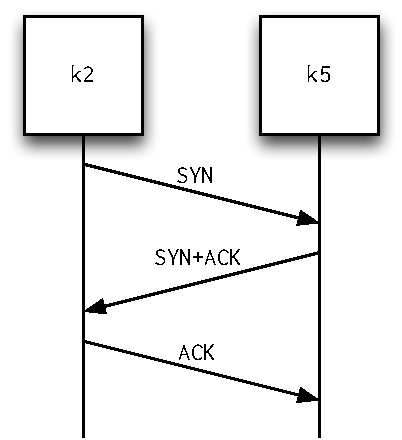
\includegraphics[width=5cm]{figury/stanowe/handshake-od-k2.pdf}}
  \qquad\qquad\qquad
  \subfloat[][]{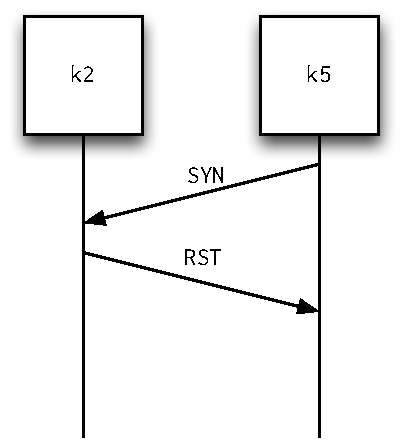
\includegraphics[width=5cm]{figury/stanowe/handshake-od-k5.pdf}}
  \caption{Wymiana komunikatów podczas \emph{handshake} przy nawiązywaniu połączenia przez maszyny po obu stronach zapory.}
  \label{fig:stanowe:handshake}
\end{figure}


\subsubsection{Wykonanie}

Wyczyszczono wszystkie reguły zapory \ipfw:

\begin{lstlisting}
k2% ipfw -q -f flush
\end{lstlisting}

Za pomocą programu \nc{} na maszynie \kpiec{} nasłuchiwano połączeń na porcie
\pos. Połączenie nawiązano z maszyny \kdwa{}. Potwierdzono, że nie ma problemu z
nawiązaniem takiego połączenia. Zbadano połączenie odwrotne. Na maszynie \kdwa{}
nasłuchiwano na porcie 6666, a nadawono z portu 80. Udało się nawiązać
połączenie.

% Nierówne są, coś ma dodatkowy margines. Jeśli suma szerokości
% minipage'y to 1\linewidth, to zajmują więcej niż linewidth.
\begin{minipage}[b]{0.4\linewidth}
\begin{lstlisting}
k2$ netcat k5 80
test
^D

k2$ netcat -l 6666
test test
k2$
\end{lstlisting}
\end{minipage}
\begin{minipage}[b]{0.12\linewidth}
  \hfill\vspace{1cm}
\end{minipage}
\begin{minipage}[b]{0.4\linewidth}
\begin{lstlisting}
k5$ netcat -l 80
test


k5$ netcat -p 80 k2 6666
test test
^D
\end{lstlisting}
\end{minipage}

Po nawiązaniu udanym nawiązaniu połączeń z obu stron rozpoczęto konfigurację
zapory. Dobrą praktyką jest rozpoczynanie konfiguracji zapory od zablokowania
całego ruchu. Niestety do prawidłowego działania maszyny niezbędne jest wiele
połączeń: \ssh{}, \texttt{LDAP}, \texttt{NAS}. Zdecydowano się na
\emph{blacklisting}. Praktyka ta polega na domyślnym przyjmowaniu wszystkich
połączeń. Jednocześnie część połączeń, zdefiniowanych na \emph{czarnej liście}
jest odrzucana. Przy tym trybie deklarowania reguł łatwo jest nieumyślnie
przeoczyć połączenie, które powinno być zablokowane i narazić sieć na atak lub
nadużycia. Dlatego nie jest to zalecany tryb konfiguracji zapory
\cite{bsd:firewall}.

W przypadku zapory stanowej można bardzo łatwo wprowadzić politykę odwrotną,
tzw. politykę białej listy. Domyślnie wszystkie pakiety przychodzące byłyby
odrzucane, natomiast pakiety wychodzące tworzyłyby nowe dynamiczne reguły.
Reguły te pozwalałyby odbiorcom pakietów na dostarczenie odpowiedzi.

Taka prosta konfiguracja zakłada, że użytkownicy w sieci chronionej firewallem
mogą być obdarzeni pełnym zaufaniem i nieograniczonym dostępem do Internetu.


\subsubsection{Konfiguracja zapory}

Na maszynie \kdwa{} zostały skonfigurowane następujące reguły zapory:

\begin{lstlisting}
00100 check-state
00150 allow tcp from any to any dst-port 80 out keep-state
00250 deny log logamount 100 ip from any to any src-port 80 in
65535 allow ip from any to any
\end{lstlisting}

Reguły \texttt{150} i \texttt{250} są podobne do tych omawianych w sekcji
\ref{sec:bezstanowe}. Zezwolono na połączenia \tcp{} wychodzące, których celem
jest dowolny adres i port \pos. Zabroniono natomiast wszystkich połączeń
przychodzących, których źródłem jest port \pos.

Dodatkowo dyrektywa \texttt{keep-state} w regule \texttt{150} instruuje zaporę,
aby dodała nowe reguły dynamiczne odpowiadające adresom i portom wykorzystanym
do połączenia \cite{bsd:firewall}. Dynamiczna reguła zostanie utworzona tylko
kiedy reguła zostanie dopasowana do połączenia.

Gdyby były to jedyne reguły, nawiązanie połączenia \tcp{} przez maszynę \kdwa{}
byłoby niemożliwe. Dzieje się tak ponieważ samo utworzenie dynamicznych reguł
nie wystarczy. Należy jeszcze dodać dyrektywę, która instruuje zaporę by
sprawdziła czy aktualny pakiet pasuje do którejś z dynamicznych reguł.

Zależało nam, aby dynamiczne reguły były sprawdzone zanim odrzucimy pakiet, z
reguły \texttt{250}. Dodano więc dyrektywę \texttt{check-state} jako regułę
\texttt{100} -- pierwszą w zestawie reguł naszej zapory.

Przy takiej konfiguracji zapora najpierw sprawdzi, czy przychodzący pakiet
pasuje do reguł dynamicznych. Jeżeli tak, zostanie on zaakceptowany. Jeżeli nie,
zapora będzie kontynuwać działanie próbując dopasować pakiet do reguł
statycznych.


\subsubsection{Testy}

Przeprowadzono testy analogiczne do tych z początku ćwiczenia.

\begin{minipage}[b]{0.4\linewidth}
\begin{lstlisting}[caption={\kdwa{}}]
k2$ netcat k5 80
test
^D

k2$ netcat -l 6666
k2$
\end{lstlisting}
\end{minipage}
\begin{minipage}[b]{0.12\linewidth}
  \hfill\vspace{1cm}
\end{minipage}
\begin{minipage}[b]{0.4\linewidth}
\begin{lstlisting}[caption={\kpiec{}}]
k5$ netcat -l 80
test
k5$ netcat -p 80 k2 6666
test test
TEST
^D
\end{lstlisting}
\end{minipage}

Można zauważyć na listingach, że osiągnęto zamierzony efekt. W drugim przypadku
testowym nie udało się nawiązać połączenia i przesłać danych do maszyny \kdwa.
